

%\myparagraph{How performance of learned heuristic changes over the value of $\gamma$}
\myparagraph{The importance of the value of $\gamma$}

Through our evaluation, we observed that the value of the hyper parameter $\gamma$ plays an important role in the performance of the learned heuristic.
Figure~\ref{fig:gamma} depicts how performance of learned heuristic changes over the hyper parameter $\gamma$.
X-axis presents the value of $\gamma$ set to learn each heuristic, and 
Y-axis presents scores that we measured for performance of each heuristic $\heuristic_{\gamma}$ according to
${\sum_{P\in\vec{P}}\projproved(F_P(\heuristic_{\gamma}(G)))}\over{\sum_{P\in\vec{P}}
  \projcost(F_P(\heuristic_{\gamma}(G)))}$ where $\projcost$ denotes analysis time(s). 
The score function present how many queries are proved per second; thereby, more precise and scalable the analysis,
higher the score.
The red dotted and black solid lines present how the scores changes over
the training programs (e.g., $\vec{P}$ = \{{\tt luindex,lusearch,antlr}\}) and validation program (e.g., $\vec{P}$ =
\{{\tt findbugs}\}), respectively.  
For the training programs, the score of the learned heuristic
increases as the higher $\gamma$ is given because the heuristic gets
fitted to the training programs.
%, and the score is a peak of the graph when the value of $\gamma$ is 0.7.
\footnote{It learned a bit bad heuristic when $\gamma$ is 0.9 in
  object-sensitivity heuristic because it is
difficult to generate specific features that satisfy such high precision
constraints; it eventually generates a general feature that include lots
of nodes.} 
The both learned heuristic, however, performs the best on the validation program when $\gamma$ is 0.5; 
\OurCtx~in Table~\ref{tbl:contextAbstraction} and \OurHeap~in Table~\ref{tbl:heapAbstraction}  corresponds to $\heuristic_{0.5}$. 
This occurs because the learned heuristics gets overfitted to the training programs as the value of $\gamma$ increases;
thus, simply increasing $\gamma$ is not an answer to show the best performance on validation and testing programs.


\begin{figure}
	\centering
	\begin{tabular}{cc}
		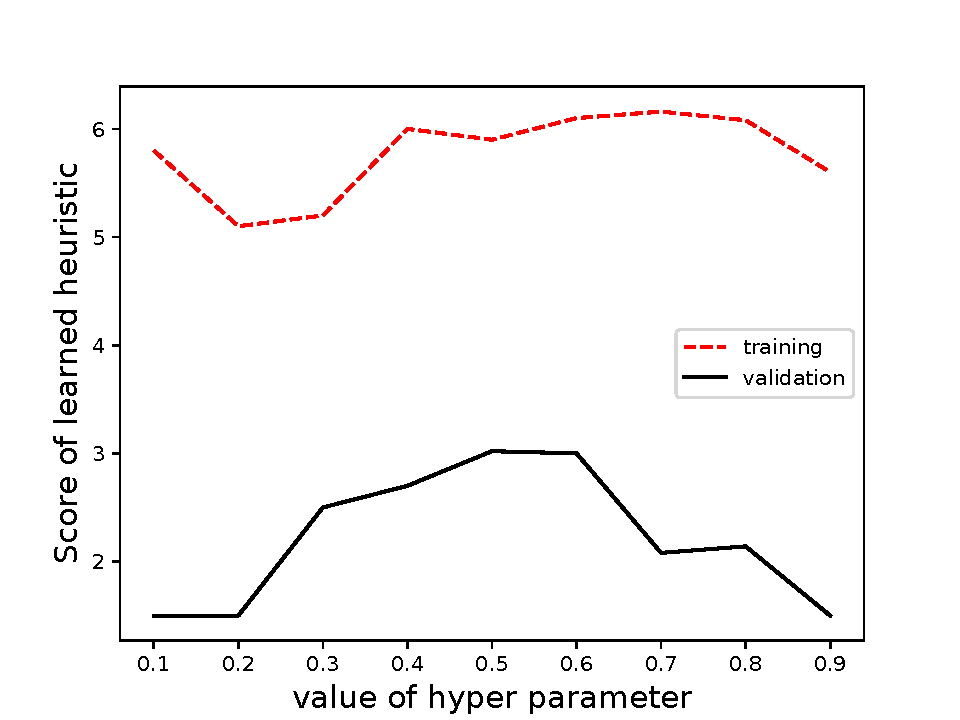
\includegraphics[width=7cm]{figures/ctx_gamma.pdf} &
		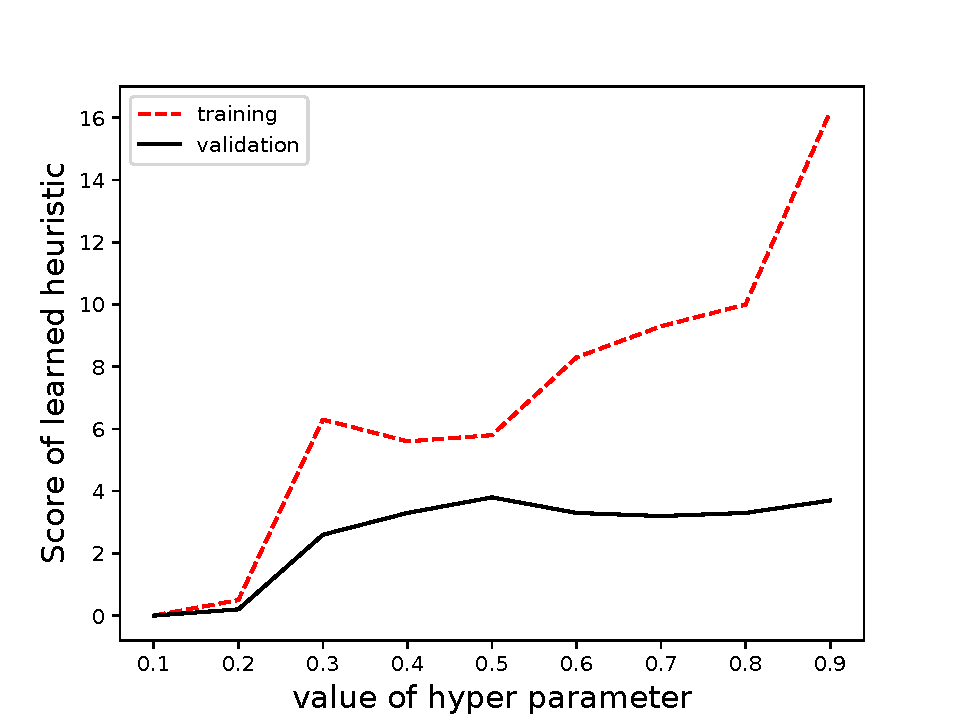
\includegraphics[width=7cm]{figures/heap_gamma.pdf}
	\end{tabular}
	\caption{How score of learned heuristic changes over the value
        of $\gamma$.}
	\label{fig:gamma}
\end{figure}




%\subsection{Learning Adequacy}

\subsection{Insights gained from Generated Features}

The generated features during learning process can provide hints on designing analysis heuristics from the graphs. 
In particular, we investigated the 96 generated features of the heap abstraction
heuristic and found two commonalities in them.
First one is that 80\% of the features have the form of $(\epsilon,\hat{n}, \hat{\vec{s}})$ where $\vec{s}$ is not $\epsilon$,
which means that we should consider successors more than predecessor when designing heap abstraction heuristics from points-to graph.
The second commonality is that $\hat{\vec{s}}$ or $\hat{n}$ tends to include an abstract
node $\aNode$ that presents nodes having lots of outgoing edges, i.e., $\aNode =
(itv,[b,\infty])$ where the number $b$ is about $3\%$ of the total nodes in a graph of a training program. 
From these observations, we manually designed a graph-based heap abstraction heuristic that
takes FPG and assigns allocation-site based heap abstraction to nodes 
that at least $3\%$ of nodes in the graph belongs to its successor
or such node exists in its successors; it assigns type-based heap abstraction to the others.
Table~\ref{tbl:principle} demonstrates the performance of the manually-crafted heuristic.
%Compared to the baseline heuristic~\AllocBased,
In comparison to the baseline \AllocBased, it reduces about 99\% of analysis cost while produces only 2\% more alarms.



Intuitively, such nodes, which have lots of successors in FPG, should
be analyzed precisely because merging the objects with others would produces lots of spurious analysis results. 
Let's assume an object which has lots of field objects. 
If we merge the object with another one which has a few field objects, it produces lots of spurious 
results that the both heaps have lots of field objects.
Such principle is related with that of \Mahjong which merges the two objects if they have the same types of successors because,
statically, an object having lots of successors is hard to have exactly the same types of successors with other objects.
Surprisingly, it is easy to find such principle through the features generated by our framework.


\begin{table}[]
\caption{Performance of manually-designed heuristic}
\label{tbl:principle}
\begin{tabular}{@{}clrr | clrr@{}}
\toprule
benchmarks               & \multicolumn{1}{c}{} & \multicolumn{1}{c}{alarms} & \multicolumn{1}{c|}{time(s)} & benchmarks                & \multicolumn{1}{c}{} & \multicolumn{1}{c}{alarms} & \multicolumn{1}{c}{time(s)} \\ \midrule
\multirow{2}{*}{luindex} & \Principle              & 374                        & 29                          & \multirow{2}{*}{lusearch} & \Principle            & 388                        & 33                          \\
                         % & \OurHeap            & 358                        & 23                          &                           & \OurHeap              & 372                        & 21                          \\
                         & \AllocBased          & 358                        & 5,475                       &                           & \AllocBased          & -                          & >10,800        \\\midrule
\multirow{2}{*}{antlr}   & \Principle              & 479                        & 44                          & \multirow{2}{*}{pmd}      & \Principle            & 886                        & 83                          \\
                         % & \OurHeap            & 463                        & 49                          &                           & \OurHeap              & 871                        & 48                          \\
                         & \AllocBased          & 463                        & 5,241                       &                           & \AllocBased          & 871                        & 9,146                       \\\midrule
\multirow{2}{*}{fop}     & \Principle            & 391                        & 41                          & \multirow{2}{*}{xalan}    & \Principle            & 548                        & 841                         \\
                         % & \OurHeap              & 376                        & 30                          &                           & \OurHeap              & 539                        & 489                         \\
                         & \AllocBased          & -                          & >10,800        &                           & \AllocBased          & -                          & >10,800        \\ \bottomrule
\end{tabular}
\end{table}




%%% Local Variables:
%%% mode: latex
%%% TeX-master: "paper"
%%% End: 